% Propiedades del documento
\documentclass[12pt]{report}

\usepackage[spanish,es-tabla]{babel}
\usepackage[utf8]{inputenc}
\usepackage[section]{placeins}
\usepackage{titlesec}
\usepackage{color}
\usepackage{graphicx}
\usepackage[a4paper,width=150mm,top=25mm,bottom=25mm,bindingoffset=6mm]{geometry}
\usepackage{fancyhdr}
\pagestyle{fancy}
\usepackage{subfig}

\usepackage{hyperref}

% Estilo de los enlaces
\hypersetup{
    colorlinks=true, % make the links colored
    linkcolor=black, % color TOC links in blue
    urlcolor=blue, % color URLs in red
    linktoc=all % 'all' will create links for everything in the TOC
}

\setlength{\headheight}{15pt}

% Quitar texto "Capítulo N"
\titleformat{\chapter}[hang]{\Huge\bfseries}{\thechapter{. }}{0pt}{\Huge\bfseries}

% Encabezado y pie de página
\fancyhead{}
\fancyhead[R]{Robot con pasillos estrechos}
\fancyfoot{}
\fancyfoot[R]{\thepage}
\fancyfoot[L]{Costel Adi Huzum \\ Andriy Byelikov}
\renewcommand{\headrulewidth}{0.4pt}
\renewcommand{\footrulewidth}{0.4pt}

% Color de los títulos
\titleformat{\chapter}{\color{red}\large}{}{0em}{\MakeUppercase}[\titlerule]

% Imágenes
\graphicspath{ {images/} }

\begin{document}

% Portada
\begin{titlepage}
    \begin{center}
 
        %\vfill
 
        %\vspace{0.8cm}
 
        
\includegraphics[width=0.4\textwidth]{logo}
        
        \vspace*{1cm}
 
        \vspace{0.5cm}
 
        \vspace{1.5cm}
        
        \Huge
        \textbf{Robot con pasillos estrechos}
        
        \vfill
 
        \Large
        
        \textbf{Sistemas Inteligentes}\\
        
        \vspace{1.5cm}
        
        Costel Adi Huzum\\
        Andriy Byelikov\\

    \end{center}
\end{titlepage}

 % Índice
\tableofcontents

% Capítulos
\chapter{Enunciado}
La práctica consiste en implementar el problema del robot que recorre el perímetro de un objeto, pero se permite la existencia de pasillos estrechos. En este caso, el robot debe ser capaz de recorrer estos pasillos sin que afecte a su recorrido. Además, en el caso de que el pasillo se encuentre bloqueado, el agente debe recorrerlo hasta al final, dar la vuelta y volver a recorrer el pasillo hasta la entrada de éste.

Finalmente, hay que implementar un interfaz agradable que permite la creación de objetos en una cuadrícula arbitraria y poner al robot en cualquier posición de la cuadrícula.

\begin{figure}[!ht]
    \centering
    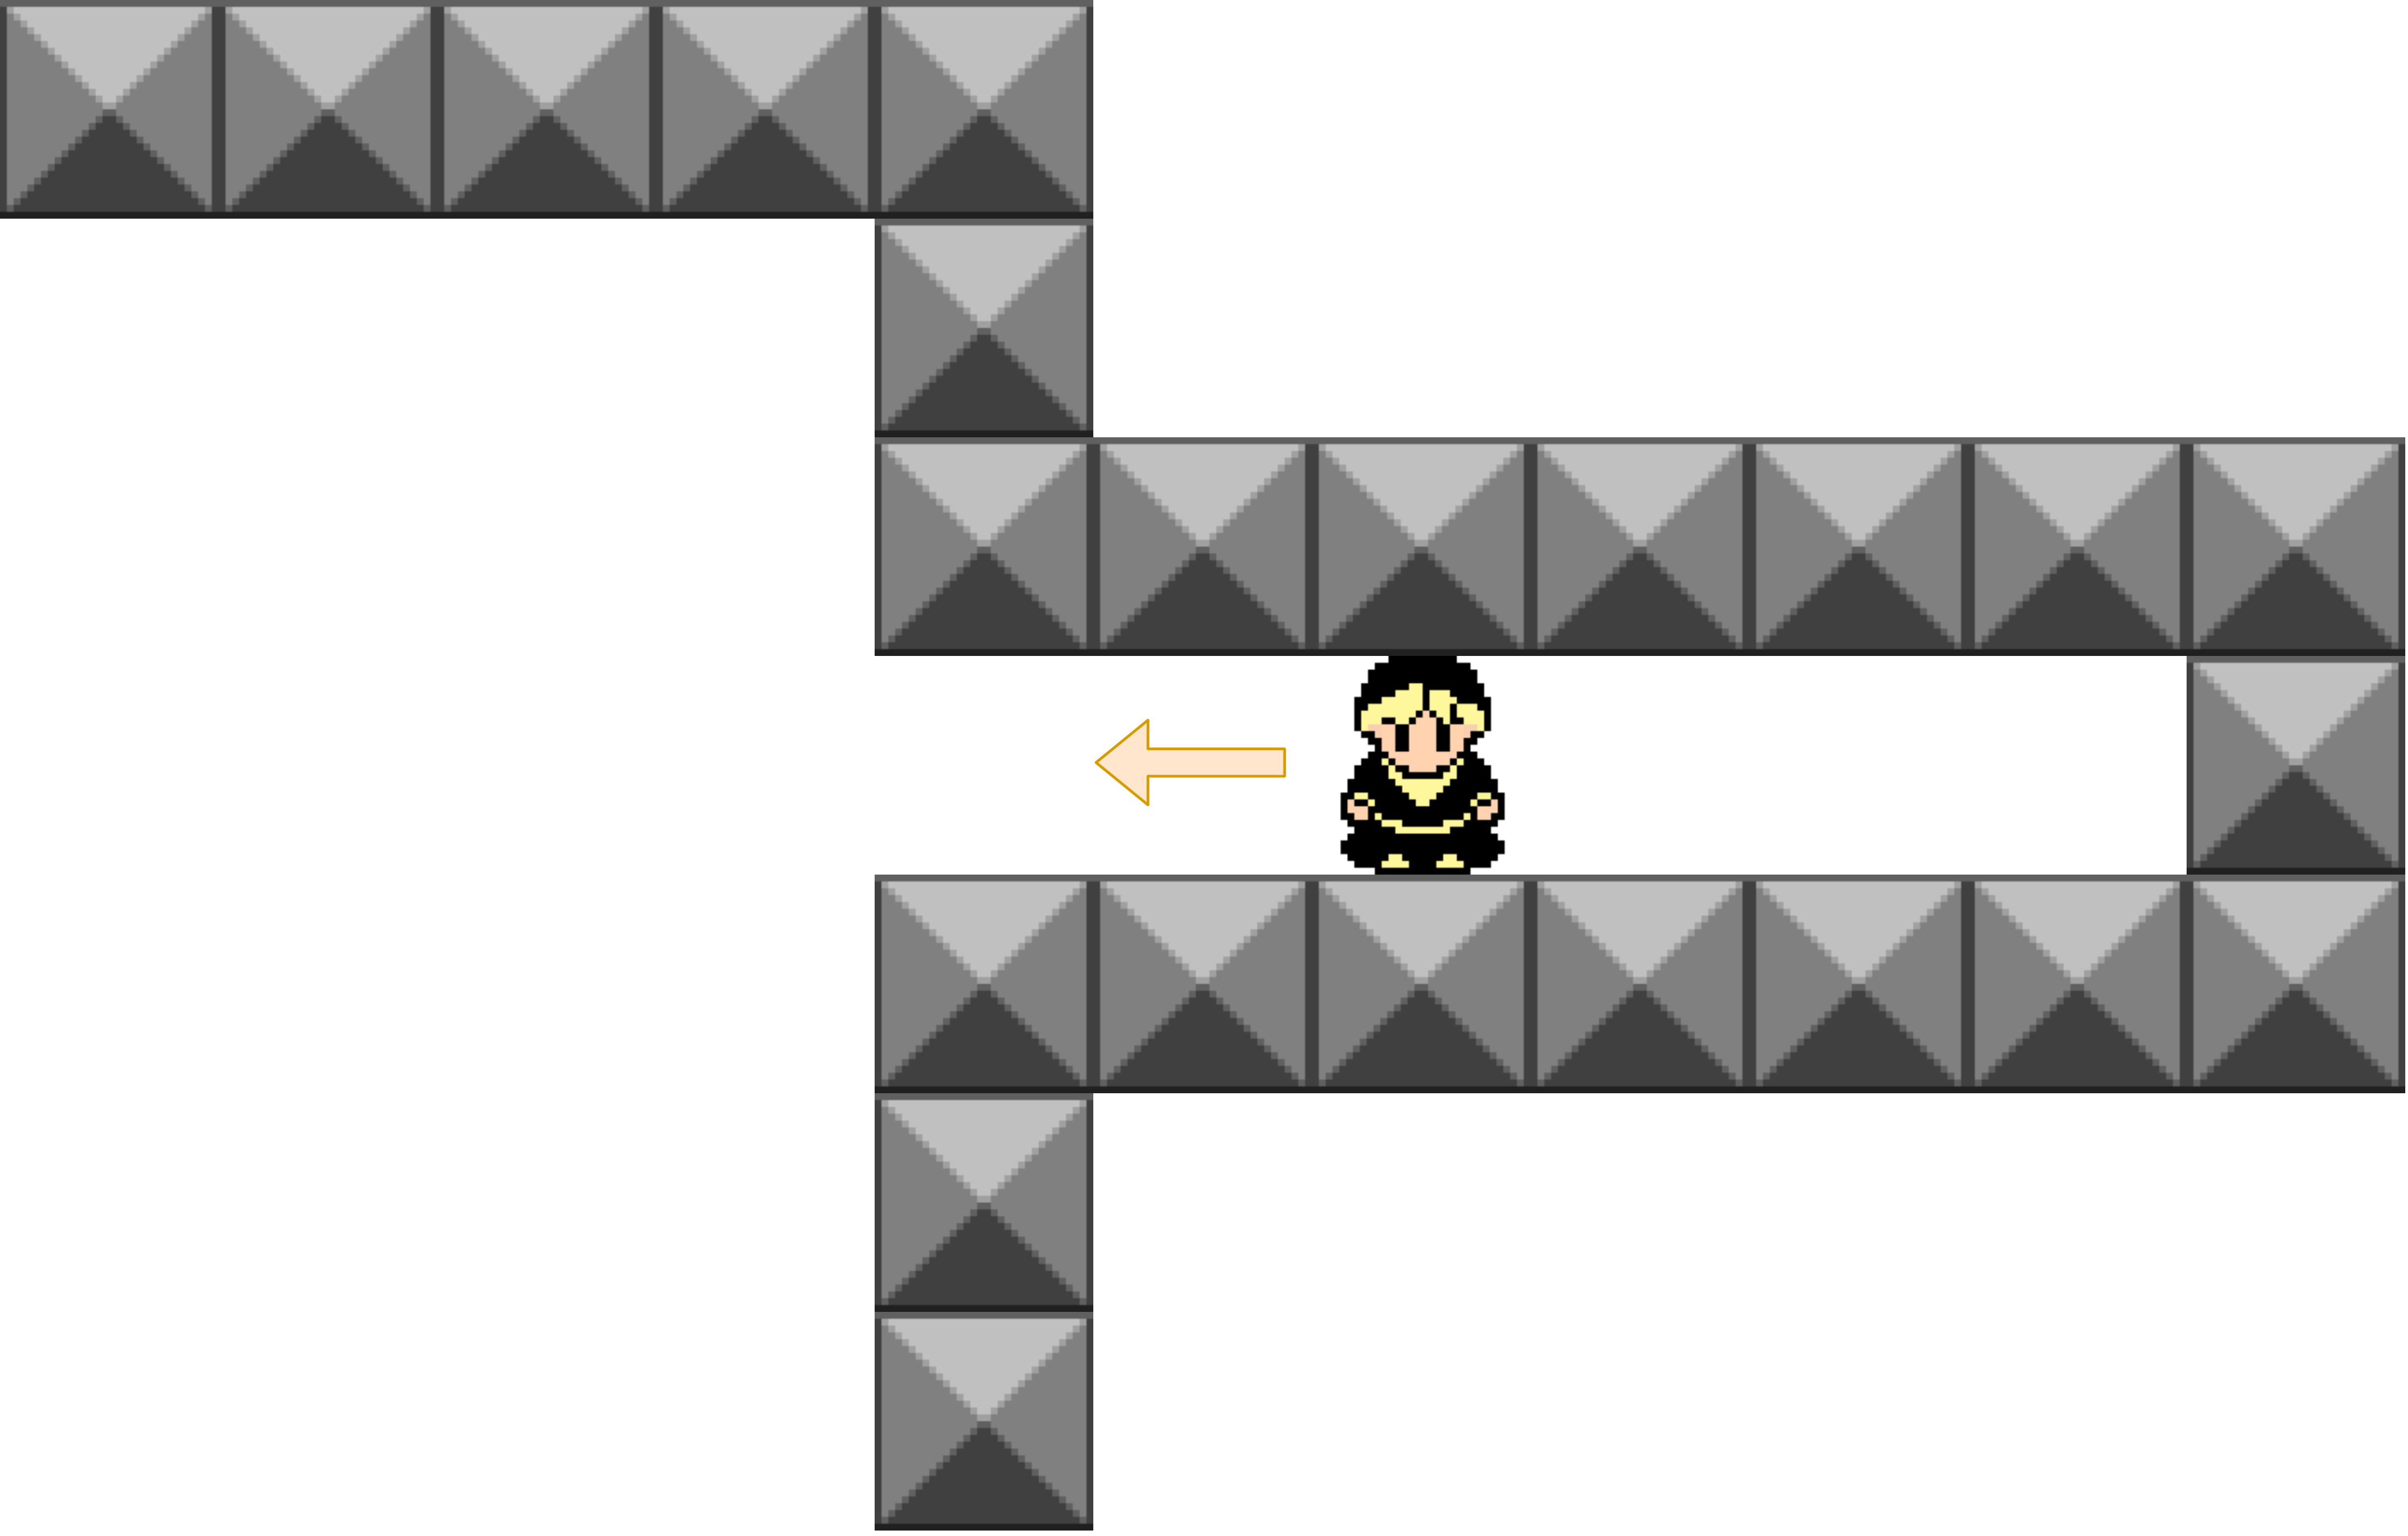
\includegraphics[width=1\textwidth]{example}
    \caption{Ejemplo de pasillo estrecho}
    \label{fig:ejemplo}
\end{figure}

\chapter{Características del agente}
\section{Componentes REAS del agente}
El agente es un agente basado en conocimiento que recibe percepciones de un entorno o ambiente sobre el cual posee información y realiza acciones en base a estas percepciones y conocimiento.

Los componentes REAS del agente son los siguientes:

\subsection{Rendimiento}

Para evaluar el buen rendimiento del agente, comprobaremos las siguientes métricas:

\begin{itemize}
    \item El agente ha sido capaz de recoger todos los tesoros posibles.
    \item El agente ha evitando todos los monstruos y precipicios.
    \item El agente ha vuelto al punto de entrada sin perecer en el intento.
\end{itemize}

\subsection{Entorno}

El agente tiene la siguiente información en la base de conocimiento sobre el entorno:
\begin{itemize}
    \item El entorno es cuadriculado.
    \item El agente conoce la orientación del entorno (sabe donde se encuentra el \emph{Norte}, \emph{Este}, \emph{Sur} y \emph{Oeste} en cada momento).
    \item El agente sabe como realizar las acciones en la dirección que ha decidido.
    \item El agente sabe cuantos proyectiles tiene para matar o escapar de monstruos.
    \item El agente conoce cuantas bombas de hedor tiene.
\end{itemize}

El agente no conoce la siguiente información del entorno (pero la puede inferir con su base de conocimiento) :
\begin{itemize}
    \item El número de monstruos y su posición.
    \item El número de tesoros y su posición.
    \item La posición de las paredes el entorno (hasta que se de un \emph{GOLPE} contra una de ellas).
    \item La posición de los hedores y brisas (hasta que se situe sobre la casilla correspondiente).
\end{itemize}

\subsection{Actuadores}

Los actuadores del agente se dividen en:

\begin{itemize}
    \item \textbf{Movimiento}: actuadores que permiten al agente explorar el entorno. Estos se realizan en sentido horario y son: \emph{DESPLAZARSE\_NORTE}, \emph{DESPLAZARSE\_ESTE}, \emph{DESPLAZARSE\_SUR} y \emph{DESPLAZARSE\_OESTE}. También se puede dar el caso en que no pueda realizar ninguna acción (al principio se encuentra rodeado de monstruos y no puede matarlos). Esta actuadores se representa como \emph{NINGUNA}.
    
    \item \textbf{Combate}: actuadores que permite al agente matar al monstruo y confundir a otros agentes lanzando bombas de hedor (hedores falsos). Estos actuadores también se realizan en orden horario (menos el de lanzar bombas de hedor, que se ejecuta aleatoriamente y es preferente a las otras acciones) y son: \emph{DISPARAR\_NORTE}, \emph{DISPARAR\_ESTE}, \emph{DISPARAR\_SUR}, \emph{DISPARAR\_OESTE} y \emph{PRODUCIR\_HEDOR}. Cada vez que se dispara un proyectil o usa una bomba de hedor se resta a su contador respectivo (definidos en el estado interno del agente). Las bombas se lanzan en la misma casilla en la que esta situada el agente (al agente no se confunde con su propia bomba porque antes de lanzar la bomba había marcado la casilla como segura) y cada un número aleatorio de ciclos.
    
    \item \textbf{Tesoro}: actuador que permite al agente recoger un tesoro y se llama \emph{RECOGER\_TESORO}.
\end{itemize}

El funcionamiento y la ejecución de estos actuadores se explicará en las reglas del agente.

\subsection{Sensores}

Los sensores del agente solo le permite obtener información de la casilla en la que se encuentre situado. Esta información son percepciones que proviene del entorno en forma de vector binario. Estas percepciones son:
\begin{itemize}
    \item \textbf{HEDOR}: hedor que proviene del monstruo o de una bomba de hedor que ha lanzado otro jugador. Los monstruos que siguen vivos producen hedor en las casillas \emph{NORTE}, \emph{ESTE}, \emph{SUR} y \emph{OESTE} respecto a la casilla que esta situado (los monstruos muertos dejan de producir hedor).
    \item \textbf{BRISA}: brisa que proviene de un precipicio. Los precipicios producen brisa en las casillas \emph{NORTE}, \emph{ESTE}, \emph{SUR} y \emph{OESTE} respecto a la casilla que esta situado.
    \item \textbf{RESPLANDOR}: el resplandor se produce en la misma casilla que el tesoro.
    \item \textbf{GOLPE}: los golpes se producen cuando un agente se choca con un muro.
    \item \textbf{GEMIDO}: los gemidos provienen cuando un monstruo muere. Los monstruos solo pueden morir cuando un proyectil impacta con él.
\end{itemize}

\section{Estado interno del agente}

El estado interno del agente se compone de:
\begin{itemize}
    \item Vector binario de percepciones: el agente utilizará este vector para inferir conocimiento sobre el entorno.
    
    \item Una representación del mapa propia: el agente utilizará este mapa para guardar cualquier información que le sea útil sobre el mapa del entorno. La representación de este mapa consiste en un conjunto de casillas, donde cada casilla es un estado. Un estado es un vector que contiene la siguiente información: si la casilla ha sido visitada; si la casilla es segura; si la casilla contiene o no monstruos o posibles monstruos; si la casilla contiene o no precipicios o posibles precipicios; si contiene brisa, hedor o tesoro; si es un muro; si la casilla se ha consumido; la dirección en que disparado el proyecto.
    
    \item Una pila de acciones: el agente guardará las acciones contrarias a las que realiza para poder volver sobre el camino que ha realizado en caso de que sea necesario.
    
    \item Acción anterior: el agente utilizará la acción anterior para mejorar el mecanismo de inferencia.
    
    \item El número de proyectiles que dispone: el entorno le proporcionará a cada agente tantos proyectiles como monstruos existen.
    
    \item El número de tesoros encontrados: el entorno utilizará este valor para determinar que agente/s han encontrado el mayor número de tesoros.
    
    \item El número de bombas de hedor restantes: cada agente empieza con 3 bombas de hedor que puede lanzar. No sabe la duración de las bombas de hedor, solo el entorno lo sabe.
    
    \item El tiempo restante para poder lanzar otra bomba de hedor: este tiempo se elije aleatoriamente entre 4 y 7 ciclos.
    
    \item El número de casillas sin consumir. Es el número de casillas adyacentes a las casillas visitadas por el agente que el agente aún no ha visitado. Sirve para que el agente se abstenga de disparar a posibles monstruos excepto cuando no pueda realizar ninguna otra acción que le permita progresar por el mapa.

\end{itemize}

\newpage
\section{Vector de características}

El vector de características (a partir de ahora, \textbf{VC}) será la herramienta que tendrá nuestro agente para realizar las acciones pertinentes en la situación en la que se encuentre. Nuestro VC será un vector binario que representará las diferentes situaciones del entorno sobre las que el agente deberá actuar:

$$ VC = (X_1,X_2,X_3, ..., X_n) $$

Ahora deberemos definir cuantos diferentes ''estados'' tendrá nuestro vector de características, esto es, cuantas diferentes situaciones puede enfrentar el agente entre sus percepciones y su estado interno. Para simplificar la lectura del vector de características, utilizaremos los siguientes símbolos:
\begin{itemize}
    \item $T_{i,j}$: Hay un tesoro en la casilla i,j.
    \item $W_{i,j}$: Hay un monstruo en la casilla i,j.
    \item $PR$: Cantidad de proyectiles que le quedan al agente.
    \item $SC$: Casillas sin consumir.
    \item $W?_{i,j}$: Posible monstruo en la casilla i,j.
    \item $M_{i,j}$: Muro en la casilla i,j.
    \item $V_{i,j}$: La casilla i,j ha sido visitada.
    \item $OK_{i,j}$: La casilla i,j es segura (no hay posibles monstruos ni posibles precipicios).
    \item $CR$: Ciclos restantes que el agente ponga una bomba de hedor.
    \item $BR$: Número de bombas de hedor restantes del agente.
\end{itemize}{}

Nuestro vector de características sería, por tanto, un vector de la forma $ VC = (X_1,X_2,X_3,X_4) $ de forma que, cada $X_i$ se define de la siguiente manera:

\begin{enumerate}
    \item $X_1 = T_{i,j}$
    \item $X_2 = CR = 0 \wedge BR > 0$
    \item $X_3 = W_{i,j} \wedge PR > 0$
    \item $X_4 = \neg H_{i,j} \wedge \neg V_{i,j} \wedge OK_{i,j}$
    \item $X_5 = W?_{i,j} \wedge SC = 0$
    \item $X_6 = W?_{i,j} \wedge SC > 0$
\end{enumerate}{}

Aunque, para especificar más en cada caso, ya que nos hará falta más adelante, podemos separar cada uno de nuestros componentes del vector de características en 4 componentes diferenciables por la casilla i,j a la que hacen referencia, dejándonos con un VC de la forma $ VC = (X_1, X_2, ..., X_{18}) $ donde cada $X_i$ se define de la siguiente manera:
\begin{enumerate}
    \item $X_1 = T_{i,j}$
    \item $X_2 = CR = 0 \wedge BR > 0$
    \item $X_3 = W_{i,j-1} \wedge PR > 0$
    \item $X_4 = W_{i+1,j} \wedge PR > 0$
    \item $X_5 = W_{i,j+1} \wedge PR > 0$
    \item $X_6 = W_{i-1,j} \wedge PR > 0$
    \item $X_7 = \neg H_{i,j-1} \wedge \neg V_{i,j-1} \wedge OK_{i,j-1}$
    \item $X_{8} = \neg H_{i+1,j} \wedge \neg V_{i+1,j} \wedge OK_{i+1,j}$
    \item $X_{9} = \neg H_{i,j+1} \wedge \neg V_{i,j+1} \wedge OK_{i,j+1}$
    \item $X_{10} = \neg H_{i-1,j} \wedge \neg V_{i-1,j} \wedge OK_{i-1,j}$
    \item $X_{11} = W?_{i,j-1} \wedge SC = 0$
    \item $X_{12} = W?_{i+1,j} \wedge SC = 0$
    \item $X_{13} = W?_{i,j+1} \wedge SC = 0$
    \item $X_{14} = W?_{i-1,j} \wedge SC = 0$
    \item $X_{15} = W?_{i,j-1} \wedge SC > 0$
    \item $X_{16} = W?_{i+1,j} \wedge SC > 0$
    \item $X_{17} = W?_{i,j+1} \wedge SC > 0$
    \item $X_{18} = W?_{i-1,j} \wedge SC > 0$
\end{enumerate}{}

\end{document}